\documentclass[t]{beamer}
\usetheme{Copenhagen}
\usepackage{amsmath, tikz, tkz-euclide, xcolor}
\usetkzobj{all}
\setbeamertemplate{headline}{} % remove toc from headers
\beamertemplatenavigationsymbolsempty

\title{Right Triangle Trigonometry}
\author{}
\date{}

\AtBeginSection[]
{
  \begin{frame}
    \frametitle{Table of Contents}
    \tableofcontents[currentsection]
  \end{frame}
}

\begin{document}

\begin{frame}{}
    \titlepage
\end{frame}

\section{Write the six trig functions of an acute angle.} 

\begin{frame}{The 3 Main Trig Ratios}

\begin{center}
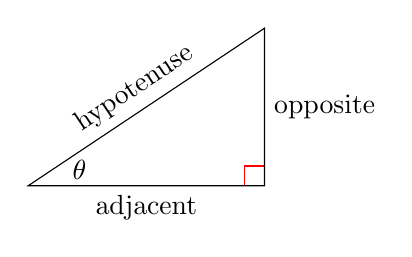
\begin{tikzpicture}
\coordinate (A) at (0,0);
\coordinate (B) at (3,2);
\coordinate (C) at (3,0);
\draw [color=red] (C) rectangle +(-0.25,0.25);
\draw (A) -- node [midway, sloped, above] {hypotenuse} (B) -- node [midway, right] {opposite} (C) -- node [midway, below] {adjacent} cycle;
\node at (A) [xshift = 0.65cm, yshift = 0.2cm] {$\theta$};
\end{tikzpicture}
\end{center}
\vspace{11pt}  
\[
\onslide<2->{\sin \theta = \dfrac{\text{opposite}}{\text{hypotenuse}}} \hspace{0.25in} 
\onslide<3->{\cos \theta = \dfrac{\text{adjacent}}{\text{hypotenuse}}} \hspace{0.25in}  
\onslide<4->{\tan \theta = \dfrac{\text{opposite}}{\text{adjacent}}}    
\]
\newline\\
\onslide<5->{We usually remember this as SOH-CAH-TOA.}
\end{frame}



\begin{frame}{Reciprocals for SOH-CAH-TOA}
\begin{center}
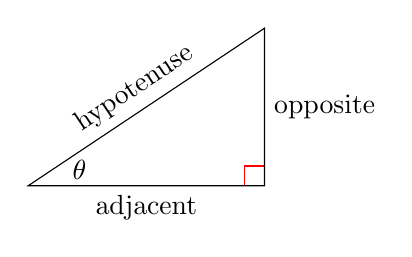
\begin{tikzpicture}
\coordinate (A) at (0,0);
\coordinate (B) at (3,2);
\coordinate (C) at (3,0);
\draw [color=red] (C) rectangle +(-0.25,0.25);
\draw (A) -- node [midway, sloped, above] {hypotenuse} (B) -- node [midway, right] {opposite} (C) -- node [midway, below] {adjacent} cycle;
\node at (A) [xshift = 0.65cm, yshift = 0.2cm] {$\theta$};
\end{tikzpicture}
\end{center}
\vspace{11pt}
\[
\onslide<2->{\csc \theta = \frac{\text{hypotenuse}}{\text{opposite}}} \quad
\onslide<3->{\sec \theta = \frac{\text{hypotenuse}}{\text{adjacent}}}  \quad
\onslide<4->{\cot \theta = \frac{\text{adjacent}}{\text{opposite}}}
\]   
\newline\\
\onslide<5->{Sometimes you may need to use the Pythagorean Theorem, $a^2+b^2=c^2$, in order to find any missing sides.}
\end{frame}

\begin{frame}{Example 1}
Find the value of each of the six trig functions of $\theta$.  \newline\\
\begin{minipage}{0.4\textwidth}
(a) \newline\\
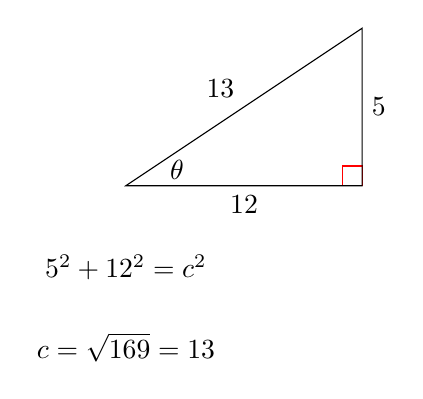
\begin{tikzpicture}
\coordinate (A) at (0,0);
\coordinate (B) at (3,2);
\coordinate (C) at (3,0);
\draw [color=red] (C) rectangle +(-0.25,0.25);
\draw (A) -- (B) -- node [midway, right] {5} (C) -- node [midway, below] {12} cycle;
\node at (A) [xshift = 0.65cm, yshift = 0.2cm] {$\theta$};
\onslide<2->{\node at (A) [below, yshift=-0.75cm] {$5^2 + 12^2 = c^2$};}
\onslide<3->{\node at (A) [below, yshift=-1.75cm] {$c = \sqrt{169}=13$};}
\onslide<4->{\node at (1.5,1) [above left] {$13$};}
\end{tikzpicture}
\end{minipage}
\begin{minipage}{0.4\textwidth}
\begin{align*}
    \onslide<5->{\sin \theta &= \frac{5}{13}}   \\[18pt]
    \onslide<6->{\cos \theta &= \frac{12}{13}}   \\[18pt]
    \onslide<7->{\tan \theta &= \frac{5}{12}}   \\
\end{align*}
\end{minipage}
\end{frame}

\begin{frame}{Example 1}
\begin{minipage}{0.4\textwidth}
(a) \newline\\
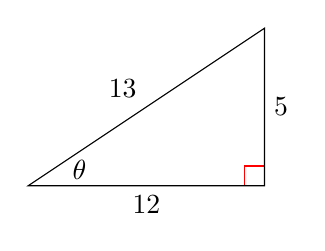
\begin{tikzpicture}
\coordinate (A) at (0,0);
\coordinate (B) at (3,2);
\coordinate (C) at (3,0);
\draw [color=red] (C) rectangle +(-0.25,0.25);
\draw (A) -- (B) -- node [midway, right] {5} (C) -- node [midway, below] {12} cycle;
\node at (A) [xshift = 0.65cm, yshift = 0.2cm] {$\theta$};
% \onslide<2->{\node at (A) [below, yshift=-0.75cm] {$5^2 + 12^2 = c^2$};}
% \onslide<3->{\node at (A) [below, yshift=-1.75cm] {$c = \sqrt{169}=13$};}
\node at (1.5,1) [above left] {$13$};
\end{tikzpicture}
\end{minipage}
\begin{minipage}{0.4\textwidth}
\begin{align*}
    \onslide<2->{\csc \theta &= \frac{13}{5}}   \\[18pt]
    \onslide<3->{\sec \theta &= \frac{13}{12}}   \\[18pt]
    \onslide<4->{\cot \theta &= \frac{12}{5}}   \\
\end{align*}
\end{minipage}
\end{frame}


\begin{frame}{Example 1}
Find the value of each of the six trig functions of $\theta$.  \newline\\
\begin{minipage}{0.45\textwidth}
(b) \newline\\
\raisebox{0.35cm}{
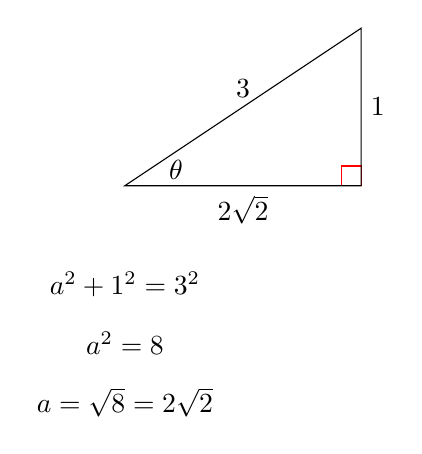
\begin{tikzpicture}
\coordinate (A) at (0,0);
\coordinate (B) at (3,2);
\coordinate (C) at (3,0);
\draw [color=red] (C) rectangle +(-0.25,0.25);
\draw (A) -- node [midway, above] {3} (B) -- node [midway, right] {1} (C) -- cycle;
\node at (A) [xshift = 0.65cm, yshift = 0.2cm] {$\theta$};
\onslide<2->{\node at (0,-1.25) {$a^2+1^2=3^2$};}
\onslide<3->{\node at (0,-2) {$a^2 = 8$};}
\onslide<4->{\node at (0,-2.75) {$a = \sqrt{8} = 2\sqrt{2}$};}
\onslide<5->{\node at (1.5,0) [below] {$2\sqrt{2}$};}
\end{tikzpicture}}
\end{minipage}
\begin{minipage}{0.4\textwidth}
\begin{align*}
    \onslide<6->{\sin \theta &= \frac{1}{3}}   \\[18pt]
    \onslide<7->{\cos \theta &= \frac{2\sqrt{2}}{3}}   \\[18pt]
    \onslide<8->{\tan \theta &= \frac{1}{2\sqrt{2}}}  
    \onslide<9->{\left(\frac{\sqrt{2}}{\sqrt{2}} \right)}
    \onslide<10->{=\frac{\sqrt{2}}{4}}\\
\end{align*}
\end{minipage}
\end{frame}

\begin{frame}{Example 1}
Find the value of each of the six trig functions of $\theta$.  \newline\\
\begin{minipage}{0.4\textwidth}
(b) \newline\\
\raisebox{0.35cm}{
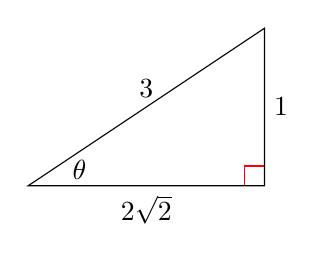
\begin{tikzpicture}
\coordinate (A) at (0,0);
\coordinate (B) at (3,2);
\coordinate (C) at (3,0);
\draw [color=red] (C) rectangle +(-0.25,0.25);
\draw (A) -- node [midway, above] {3} (B) -- node [midway, right] {1} (C) -- cycle;
\node at (A) [xshift = 0.65cm, yshift = 0.2cm] {$\theta$};
\node at (1.5,0) [below] {$2\sqrt{2}$};
\end{tikzpicture}}
\end{minipage}
\begin{minipage}{0.4\textwidth}
\begin{align*}
    \onslide<2->{\csc \theta &= \frac{3}{1} = 3}   \\[18pt]
    \onslide<3->{\sec \theta &= \frac{3}{2\sqrt{2}}} \onslide<4->{\left(\frac{\sqrt{2}}{\sqrt{2}}\right)} 
    \onslide<5->{ = \frac{3\sqrt{2}}{4}}   \\[18pt]
    \onslide<6->{\cot \theta &= \frac{2\sqrt{2}}{1}=2\sqrt{2}}  
\end{align*}
\end{minipage}
\end{frame}


\section{Find the exact trig function values for special right triangles.}

\begin{frame}{45-45-90 Triangles}

45-45-90 triangles (also known as \textit{isosceles right triangles}) can be created by drawing a diagonal across a square:

\begin{center}
    \begin{tikzpicture}
    \tkzDefPoints{0/0/A, 3/0/B, 3/3/C, 0/3/D}
    \tkzDrawPolygon(A,B,C,D)
    \tkzMarkRightAngle[color=red](A,B,C)
    \tkzDrawSegment[dashed](A,C)
    \tkzLabelAngle[pos=0.75](B,A,C){$45^\circ$}
    \tkzLabelAngle[pos=0.75](B,C,A){$45^\circ$}
    \end{tikzpicture}
\end{center}

\end{frame} 

\begin{frame}{45-45-90 Triangles}
Since each side of a square is the same length, we can use whatever length we want. For simplicity, we will use a length of 1.  \newline\\ \pause

The diagonal of the square can be found by using Pythagorean Theorem:  \pause

\begin{center}
    \begin{tikzpicture}
    \tkzDefPoints{0/0/A, 3/0/B, 3/3/C}
    \tkzDrawPolygon(A,B,C)
    \tkzMarkRightAngle[color=red](A,B,C)
    \tkzLabelAngle[pos=0.75](B,A,C){$45^\circ$}
    \tkzLabelAngle[pos=0.75](B,C,A){$45^\circ$}
    \tkzLabelSegment[right](B,C){1}
    \tkzLabelSegment[below](A,B){1}
    \tkzLabelSegment[above left, midway](A,C){$\sqrt{2}$}
    \end{tikzpicture}
\end{center}
\end{frame}

\begin{frame}{Example 2}
Find the exact values of the six trig ratios for $45^\circ$. \newline\\
\begin{minipage}{0.4\textwidth}
\begin{tikzpicture}
    \tkzDefPoints{0/0/A, 3/0/B, 3/3/C}
    \tkzDrawPolygon(A,B,C)
    \tkzMarkRightAngle[color=red](A,B,C)
    \tkzLabelAngle[pos=0.75](B,A,C){$45^\circ$}
    \tkzLabelAngle[pos=0.75](B,C,A){$45^\circ$}
    \tkzLabelSegment[right](B,C){1}
    \tkzLabelSegment[below](A,B){1}
    \tkzLabelSegment[above left, midway](A,C){$\sqrt{2}$}
    \end{tikzpicture}
\end{minipage}
\begin{minipage}{0.5\textwidth}
\begin{align*}
    \onslide<2->{\sin 45^\circ &= \frac{1}{\sqrt{2}}} \\[11pt]
    \onslide<3->{&= \frac{1}{\sqrt{2}}\frac{\sqrt{2}}{\sqrt{2}} = \frac{\sqrt{2}}{2}} \\[11pt]
    \onslide<4->{\cos45^\circ &= \frac{1}{\sqrt{2}} = \frac{\sqrt{2}}{2}} \\[11pt]
    \onslide<5->{\tan 45^\circ &= \frac{1}{1} = 1}
\end{align*}
\end{minipage}
\end{frame}

\begin{frame}{Example 2}
\begin{minipage}{0.4\textwidth}
\begin{tikzpicture}
    \tkzDefPoints{0/0/A, 3/0/B, 3/3/C}
    \tkzDrawPolygon(A,B,C)
    \tkzMarkRightAngle[color=red](A,B,C)
    \tkzLabelAngle[pos=0.75](B,A,C){$45^\circ$}
    \tkzLabelAngle[pos=0.75](B,C,A){$45^\circ$}
    \tkzLabelSegment[right](B,C){1}
    \tkzLabelSegment[below](A,B){1}
    \tkzLabelSegment[above left, midway](A,C){$\sqrt{2}$}
    \end{tikzpicture}
\end{minipage}
\begin{minipage}{0.5\textwidth}
\begin{align*}
    \onslide<2->{\csc 45^\circ &= \frac{\sqrt{2}}{1} = \sqrt{2}} \\[18pt]
    \onslide<3->{\sec45^\circ &= \frac{\sqrt{2}}{1} = \sqrt{2}} \\[18pt]
    \onslide<4->{\cot 45^\circ &= \frac{1}{1} = 1}    \\[11pt]
\end{align*}
\end{minipage}    
\onslide<5->{\emph{Note}: Your answers from the above example will be the same if you replace $45^\circ$ with $\frac{\pi}{4}$.}
\end{frame}

\begin{frame}{30-60-90 Triangles}
    We can create a 30-60-90 triangle by drawing an altitude in an equilateral triangle.

\begin{center}
    \begin{tikzpicture}
    \tkzDefPoints{0/0/A, 4/0/B}
    \tkzDefPoint(60:4){C}
    \tkzDrawPolygon(A,B,C)
    \tkzDefMidPoint(A,B)
        \tkzGetPoint{D}
    \tkzDrawSegment[dashed](D,C)
    \tkzMarkRightAngle[color=red](A,D,C)
    \tkzLabelAngle[pos=0.5](D,A,C){$60^\circ$}
    \tkzLabelAngle[pos=1](D,C,A){$30^\circ$}
    \end{tikzpicture}
\end{center}
\end{frame}

\begin{frame}{30-60-90 Triangles}
Recall that the altitude of an equilateral triangle bisects one of the sides.   \newline\\    \pause

Rather than use a length of 1 for the sides of the equilateral triangle, we will use a length of 2 (if only to avoid using fractions). \newline\\ \pause

\begin{center}
    \begin{tikzpicture}
    \tkzDefPoints{0/0/A, 4/0/B}
    \tkzDefPoint(60:4){C}
    \tkzDrawPolygon(A,B,C)
    \tkzDefMidPoint(A,B)
        \tkzGetPoint{D}
    \tkzDrawSegment[dashed](D,C)
    \tkzMarkRightAngle[color=red](A,D,C)
    \tkzLabelAngle[pos=0.5](D,A,C){$60^\circ$}
    \tkzLabelAngle[pos=1](D,C,A){$30^\circ$}
    \tkzLabelSegment[below](A,D){1}
    \tkzLabelSegment[below](D,B){1}
    \tkzLabelSegment[midway, above left](A,C){2}
    \tkzLabelSegment[midway, above right](B,C){2}
    \end{tikzpicture}
\end{center}
\end{frame}

\begin{frame}{30-60-90 Triangles}
We can use the Pythagorean Theorem to find the length of the altitude, $\sqrt{3}$:

\begin{center}
    \begin{tikzpicture}
    \tkzDefPoints{0/0/A, 2/0/B}
    \tkzDefPoint(60:4){C}
    \tkzDrawPolygon(A,B,C)
    \tkzMarkRightAngle[color=red](A,B,C)
    \tkzLabelAngle[pos=0.5](B,A,C){$60^\circ$}
    \tkzLabelAngle(B,C,A){$30^\circ$}
    \tkzLabelSegment[below](A,B){1}
    \tkzLabelSegment[right](B,C){$\sqrt{3}$}
    \tkzLabelSegment[midway, above left](A,C){2}
    \end{tikzpicture}
\end{center}
\end{frame}

\begin{frame}{Example 3}
Find the exact values of the six trig ratios for $60^\circ$. \newline\\
\begin{minipage}{0.4\textwidth}
\begin{tikzpicture}
    \tkzDefPoints{0/0/A, 2/0/B}
    \tkzDefPoint(60:4){C}
    \tkzDrawPolygon(A,B,C)
    \tkzMarkRightAngle[color=red](A,B,C)
    \tkzLabelAngle[pos=0.5](B,A,C){$60^\circ$}
    \tkzLabelAngle(B,C,A){$30^\circ$}
    \tkzLabelSegment[below](A,B){1}
    \tkzLabelSegment[right](B,C){$\sqrt{3}$}
    \tkzLabelSegment[midway, above left](A,C){2}
    \end{tikzpicture}
\end{minipage}
\begin{minipage}{0.5\textwidth}
\begin{align*}
    \onslide<2->{\sin 60^\circ &= \frac{\sqrt{3}}{2}} \\[11pt]
    \onslide<3->{\cos 60^\circ &= \frac{1}{2}} \\[11pt]
    \onslide<4->{\tan 60^\circ &= \frac{\sqrt{3}}{1} = \sqrt{3}}
\end{align*}
\end{minipage}
\end{frame}

\begin{frame}{Example 3}
\begin{minipage}{0.4\textwidth}
\begin{tikzpicture}
    \tkzDefPoints{0/0/A, 2/0/B}
    \tkzDefPoint(60:4){C}
    \tkzDrawPolygon(A,B,C)
    \tkzMarkRightAngle[color=red](A,B,C)
    \tkzLabelAngle[pos=0.5](B,A,C){$60^\circ$}
    \tkzLabelAngle(B,C,A){$30^\circ$}
    \tkzLabelSegment[below](A,B){1}
    \tkzLabelSegment[right](B,C){$\sqrt{3}$}
    \tkzLabelSegment[midway, above left](A,C){2}
    \end{tikzpicture}
\end{minipage}
\begin{minipage}{0.5\textwidth}
\begin{align*}
    \onslide<2->{\csc 60^\circ &= \frac{2}{\sqrt{3}}} \\[11pt]
    \onslide<3->{&= \frac{2}{\sqrt{3}}\frac{\sqrt{3}}{\sqrt{3}} = \frac{2\sqrt{3}}{3}} \\[11pt]
    \onslide<4->{\sec 60^\circ &= \frac{2}{1} = 2} \\[11pt]
    \onslide<5->{\cot 60^\circ &= \frac{1}{\sqrt{3}}} \\[11pt]
    \onslide<6->{&= \frac{1}{\sqrt{3}}\frac{\sqrt{3}}{\sqrt{3}} = \frac{\sqrt{3}}{3}}
\end{align*}
\end{minipage}
\end{frame}

\begin{frame}{Example 4}
Find the exact values of the six trig ratios for $30^\circ$. \newline\\
\begin{minipage}{0.4\textwidth}
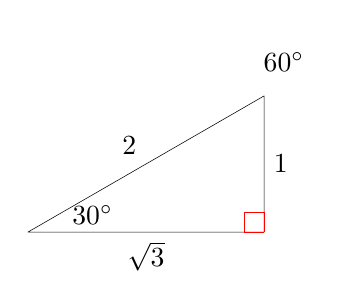
\begin{tikzpicture}
    \tkzDefPoints{0/0/A, 3/0/B, 3/1.73/C}
    \tkzDrawPolygon(A,B,C)
    \tkzMarkRightAngle[color=red](A,B,C)
    \tkzLabelAngle[pos=0.85](B,A,C){$30^\circ$}
    \tkzLabelAngle[pos=0.5](B,C,A){$60^\circ$}
    \tkzLabelSegment[below](A,B){$\sqrt{3}$}
    \tkzLabelSegment[right](B,C){1}
    \tkzLabelSegment[midway, above left](A,C){2}
    \end{tikzpicture}
\end{minipage}
\begin{minipage}{0.5\textwidth}
\begin{align*}
    \onslide<2->{\sin 30^\circ &= \frac{1}{2}} \\[11pt]
    \onslide<3->{\cos 30^\circ &= \frac{\sqrt{3}}{2}} \\[11pt]
    \onslide<4->{\tan 30^\circ &= \frac{1}{\sqrt{3}} = \frac{\sqrt{3}}{3}}
\end{align*}
\end{minipage}
\end{frame}

\begin{frame}{Example 4}
\begin{minipage}{0.4\textwidth}
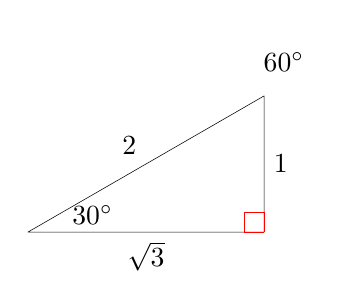
\begin{tikzpicture}
    \tkzDefPoints{0/0/A, 3/0/B, 3/1.73/C}
    \tkzDrawPolygon(A,B,C)
    \tkzMarkRightAngle[color=red](A,B,C)
    \tkzLabelAngle[pos=0.85](B,A,C){$30^\circ$}
    \tkzLabelAngle[pos=0.5](B,C,A){$60^\circ$}
    \tkzLabelSegment[below](A,B){$\sqrt{3}$}
    \tkzLabelSegment[right](B,C){1}
    \tkzLabelSegment[midway, above left](A,C){2}
    \end{tikzpicture}
\end{minipage}
\begin{minipage}{0.5\textwidth}
\begin{align*}
    \onslide<2->{\csc 30^\circ &= \frac{2}{1} = 2} \\[11pt]
    \onslide<3->{\sec 30^\circ &= \frac{2}{\sqrt{3}} = \frac{2\sqrt{3}}{3}} \\[11pt]
    \onslide<4->{\cot 30^\circ &= \frac{\sqrt{3}}{1} = \sqrt{3}}  \\[11pt]
\end{align*}
\end{minipage}    
\end{frame}

\begin{frame}{Cofunctions}
Notice how $\sin 30^\circ = \cos 60^\circ$, $\tan 30^\circ = \cot 60^\circ$, etc. This is because these ratios are \alert{cofunctions}.   \newline\\  \pause

Any pair of trig functions $f$ and $g$ for which
\[
f(\theta) = g\left(90^\circ - \theta\right)
\]
and vice versa are \textbf{cofunctions}.
\end{frame}

\section{Find missing side lengths in right triangles.}

\begin{frame}{Finding Missing Sides}
You can use SOH-CAH-TOA and your calculator to find missing sides in right triangles.
\end{frame}

\begin{frame}{Example 5}
Find the value of $x$. Round your answer to 2 decimal places. \newline\\
\begin{center}
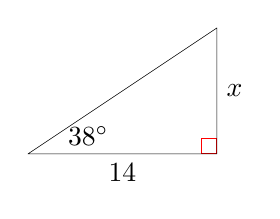
\begin{tikzpicture}[scale=0.8]
    \tkzDefPoints{0/0/A, 3/0/B, 3/2/C}
    \tkzMarkRightAngle[color=red](C,B,A)
    \tkzDrawPolygon(A,B,C)
    \tkzLabelAngle[](B,A,C){$38^\circ$}
    \tkzLabelSegment[right](B,C){$x$}
    \tkzLabelSegment[below](A,B){14}
\end{tikzpicture}
\end{center}
\begin{align*}
    \onslide<2->{\tan 38^\circ &= \frac{x}{14}} \\[10pt]
    \onslide<3->{0.7813 &= \frac{x}{14}} \\[10pt]
    \onslide<4->{x &= 14(0.7813) \approx 10.94}
\end{align*}
\end{frame}
\end{document}
